\chapter{Outlier Detection}
\section{Outlier Types}\label{section:outlier-detection}
Outliers can be categorized as point outliers or subsequence outliers.
\subsubsection{Point Outliers}
A point outlier is a single datapoint that strongly varies from the usual trend of the datapoints. \cite{blazquez-garciaReviewOutlierAnomaly2020} Examples of three point outliers are shown in \autoref{figure:point-outliers}.
\begin{figure}[h]
  \centering
  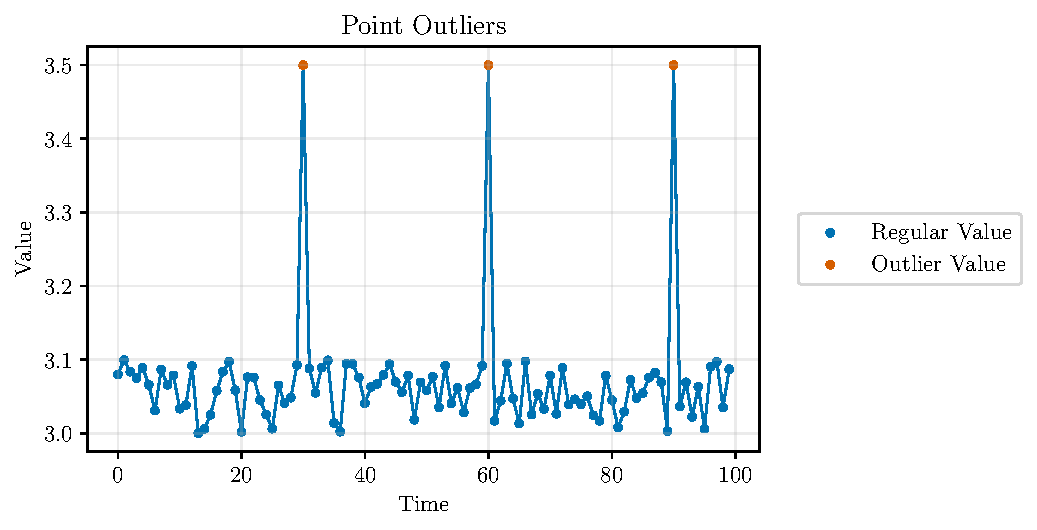
\includegraphics{./plots/pdfs/point_outliers.pdf}
  \caption{Examples of three point outliers}
  \label{figure:point-outliers}
\end{figure}

\subsubsection{Subsequence outliers}
Subsequence outliers are multiple consecutive datapoints that strongly vary from the usual trend of the datapoints. \cite{blazquez-garciaReviewOutlierAnomaly2020} In \autoref{figure:subsequence-outliers} examples of subsequence outliers are shown.
\newline\newline
\begin{figure}[h]
  \centering
  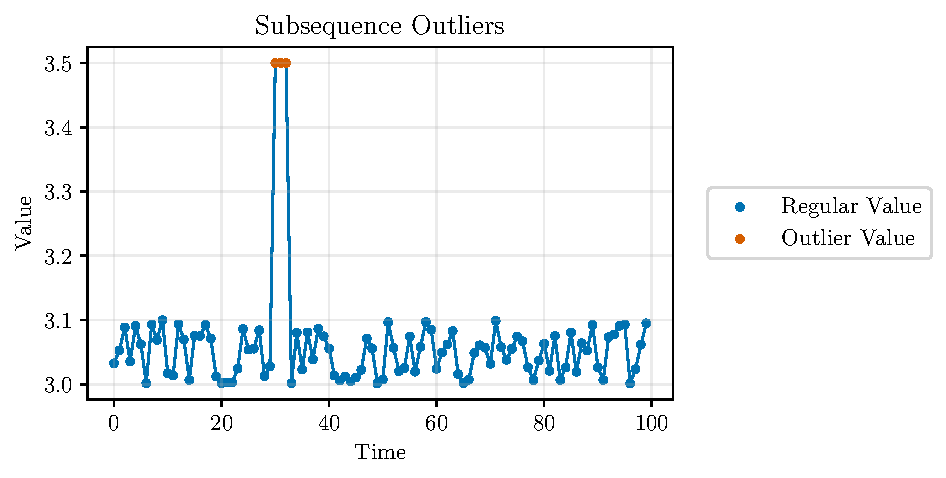
\includegraphics{./plots/pdfs/subsequence_outliers.pdf}
  \caption{Examples of three subsequence outliers}
  \label{figure:subsequence-outliers}
\end{figure}
Furthermore outliers can be divided into local and global outliers. 
\subsubsection{Local Outliers}
A local outlier has a greater variance to its direct neighbouring datapoints (previous and next one) \cite{blazquez-garciaReviewOutlierAnomaly2020} In \autoref{figure:local-point-outliers} and \autoref{figure:local-subsequence-outliers} examples of local outliers are shown. The first two outliers in \autoref{figure:local-point-outliers} have a great variance towards it direct neighbours, however not to the values from Time 60 onwards.
\begin{figure}[H]
  \centering
  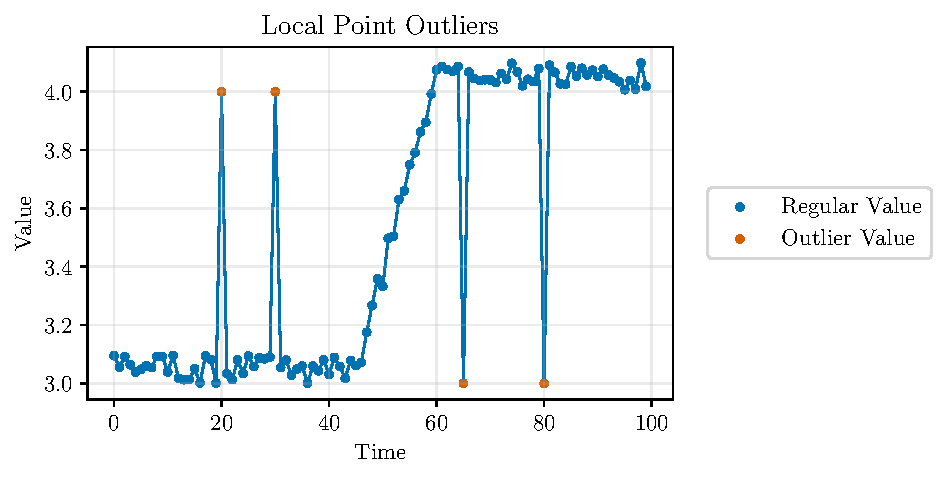
\includegraphics{./plots/pdfs/local_point_outliers.pdf}
  \caption{Examples of four local point outliers}
  \label{figure:local-point-outliers}
\end{figure}
\begin{figure}[H]
  \centering
  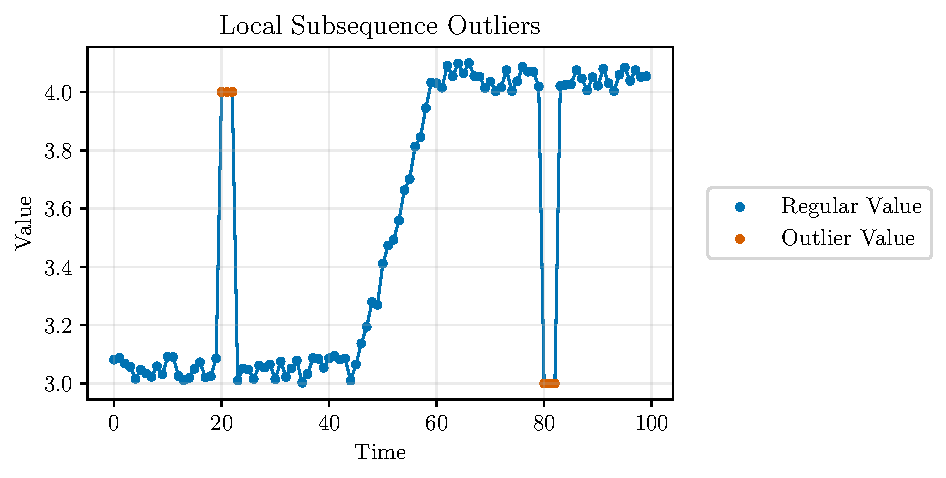
\includegraphics{./plots/pdfs/local_subsequence_outliers.pdf}
  \caption{Examples of six local subsequence outliers}
  \label{figure:local-subsequence-outliers}
\end{figure}
\subsubsection{Global Outliers}
Whereas a global outlier varies more in regard to all datapoints. \autoref{figure:point-outliers}, \ref{figure:subsequence-outliers} and \ref{figure:global-point-outliers} show picture examples of global outliers.
\cite{blazquez-garciaReviewOutlierAnomaly2020}
\begin{figure}[H]
  \centering
  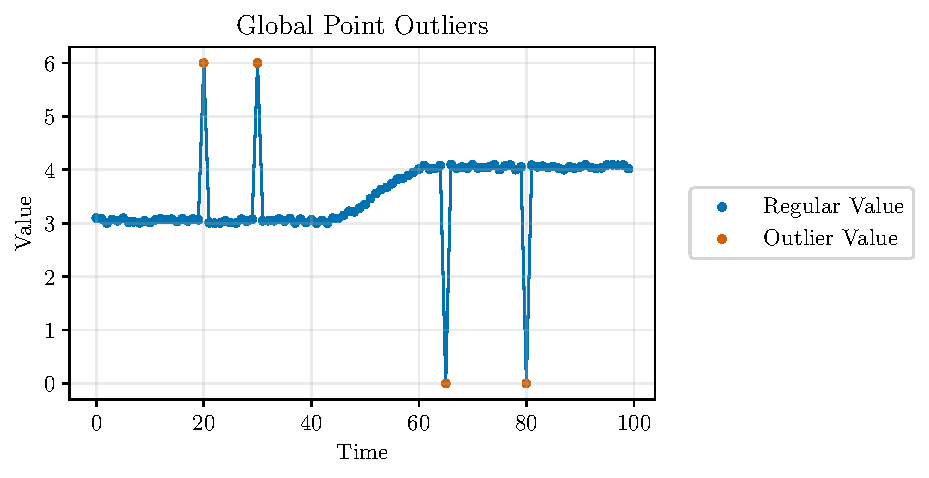
\includegraphics{./plots/pdfs/global_point_outliers.pdf}
  \caption{Examples of four global point outliers}
  \label{figure:global-point-outliers}
\end{figure}

\section{Outlier Detection Approaches}\label{section:outlier-detection-approaches}
Outlier detection methods can be divided into the following groups
\subsubsection{Statistical}
For statistical outlier detection, historical data is taken to develop a model that pictures the expected behavior of the data. An example of a statistical outlier detection is the threshold based method described in \autoref{section:threshold-based-outlier-detection} \cite{cookAnomalyDetectionIoT2020, giannoniAnomalyDetectionModels2018}

\subsubsection{Distance based}
For this approach a distance metric needs to be defined, (e.g. Euclidean distance). Then each datapoint is compared to the data preceding it. The greater the distance between the current and previous datapoints the greater the probability of an anomaly. \cite{cookAnomalyDetectionIoT2020, giannoniAnomalyDetectionModels2018, chandolaAnomalyDetectionSurvey2009}

\subsubsection{Clustering}
Clustering also requires a set of historical data in order to train the clustering model. Usually the data is clustered into two clusters: normal data and anomalous data. Depending on the distance of a new datapoint to the "normal" and the "anomalous" cluster it is classified.
\cite{cookAnomalyDetectionIoT2020, giannoniAnomalyDetectionModels2018, chandolaAnomalyDetectionSurvey2009}
\subsubsection{Predictive}
In this approach a prediction model needs to be developed, based on previous data. The prediction of this model is then compared with the actual datapoint (new data, which was not used in training the model). If the actual datapoint differs too much from the prediction it is labelled as an anomaly. \cite{cookAnomalyDetectionIoT2020, giannoniAnomalyDetectionModels2018}


\subsubsection{Ensemble}
as the word ensemble suggests, this is a collection of outlier detection methods that use a specific vote mechanism to determine whether a datapoint is faulty or normal. For example using the majority vote system and a statistical, distance based and predictive method to detect outliers. If at least two methods flag a datapoint as an outlier the ensemble reports it as an outlier as well. If only one method reports it as an outlier the ensemble does not flag it as an anomaly.
\cite{cookAnomalyDetectionIoT2020}

\section{Threshold based Outlier Detection}\label{section:threshold-based-outlier-detection}
Threshold based detection methods are able to identify outliers based on a given threshold $\tau$. These Methods can be described with the following formula
$$
  |x_t - \hat{x}_t | > \tau \text{ \cite{blazquez-garciaReviewOutlierAnomaly2020}}
$$
Where $x_t$ is the actual value and $\hat{x}_t$ is the expected value and $\tau$ is a given threshold.\\
Methods to calculate $\hat{x}_t$ will be described in the following sections. Furthermore $\hat{x}_t$ can be calculated using the entire data series or with subsets (of equal length) of the entire data series. This means $\hat{x}_t$ can be either calculated for the whole data series or for just a segment.\\
Depending on the sensitivity wanted for outlier detection an appropriate $\tau$ needs to be chosen. The greater $\tau$ is the fewer outliers will be detected. The smaller $\tau$ is the more outliers will be identified.  \cite{blazquez-garciaReviewOutlierAnomaly2020}

\subsubsection{Mean}
$$
  \text{mean} = \bar{x} = \frac{1}{n} \sum^n_{t=0}x_t
$$
Where $n$ is the total number of samples. Using the mean as an expected value is not robust to outliers, because the median is not as robust as the mean in hindsight to outliers. To calculate the mean all datapoints of a series must be summed up and then divided by the number of datapoints.
\subsubsection{Median}
If $n$ is odd:
$$
  median(x) = x_{(n+1)/2}
$$
If $n$ is even:
$$
  median(x) = \frac{x_{n/2} + x_{(n+1)/2}}{2}
$$
Where $x$ is a dataset of $n$ elements ordered from smallest to largest\\
($x_1 \leq x_2 \leq x_3 \leq \ldots \leq x_{n-2} \leq x_{n-1} \leq x_n$)
\cite{blazquez-garciaReviewOutlierAnomaly2020}
To calculate the median all values must be sorted from smallest to largest. If the number of datapoints is odd then the most center datapoint is the Median (e.g. if the series consist of 7 values the third value is the median). If the number of datapoints is even then the median is the mean of the two datapoints in the center.
\subsubsection{Median Absolute Deviation (\ac{MAD})}
The Median Absolute Deviation 
$$
  MAD = median(|x_t - median(x)|)
$$
$MAD$ is a more robust (regarding outliers) way to calculate the deviation of a dataset. To calculate the $MAD$ firstly the median of the dataset must be calculated. Then the absolute difference between $x_t$ and the median of the dataset is calculated. The Median of all differences results in the $MAD$
\cite{leysDetectingOutliersNot2013, mehrangOutlierDetectionWeight2015}

\section{Outlier Detection using z-score}
\label{section:outlier-detection-z-score}
The z-score, also known as the standard score, is the factor of how many standard deviations a datapoint differs from the mean. Using standard score to detect outliers works best, when the data is distributed normally. Because then it can be assumed, that e.g. the top and bottom 0.5\% are outliers and therefore every value with $|z| > \approx 2.576$ can be classified as an outlier. %2.5758293035489
A visual representation of the z-score in a normal distribution is shown in \autoref{figure:normal-distribution}
\begin{equation*}
  z_t = \frac{x_t - \mu}{\sigma}
\end{equation*}

Where $\mu$ is the mean of the dataset and $\sigma$ is the standard deviation. When the mean and the standard deviation of the entire dataset is now known the mean and the standard deviation of a known sample can be used.
\cite{DetectionSpatialOutlier, teschlSpezielleStetigeVerteilungen2014, rousseeuwAnomalyDetectionRobust2018}
\begin{figure}[H]
  \centering
  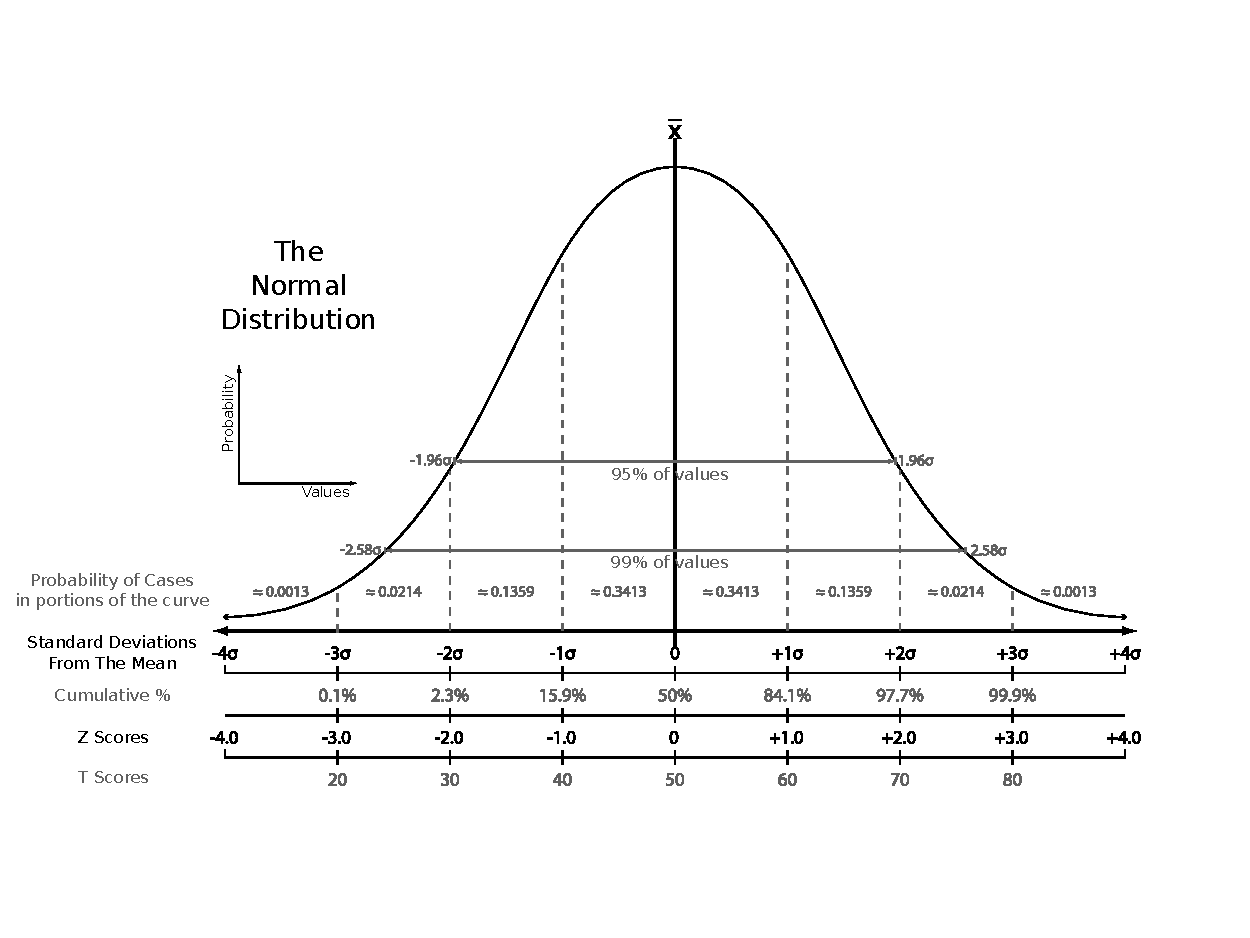
\includegraphics[width=\textwidth]{./pics/The_Normal_Distribution.pdf}
  \caption{Standard Score in a normal distribution\cite{StandardScore2022}}
  \label{figure:normal-distribution}
\end{figure}
\begin{equation*}
  \sigma = s = \sqrt{\frac{1}{n-1}\sum^n_{i=1}{(x_i - \bar{x})^2}}
\end{equation*}
\cite{teschlSpezielleStetigeVerteilungen2014, rousseeuwAnomalyDetectionRobust2018}
\par
To check whether the value $x_t$ is an outlier the absolute of its z-score is compared against a threshold ($\tau$) and if the absolute value of the z-score exceeds the threshold $x_t$ is classified as an outlier.
\begin{equation*}
  |z_t| > \tau
\end{equation*}
\section{Outlier Detection using modified z-score}
Because the mean and standard deviation are not robust towards outliers the z-score can be modified to use more robust metrics for the expected value and the variation of the values. To make the outlier detection with the z-score more robust the mean can be replaced with the median and the standard deviation with the \ac{MAD} or the \ac{MADN}. A possible formula for a modified z-score, as described in \cite{baeOutlierDetectionSmoothing2019}, could be:
\begin{equation*}
  m_t = \frac{|x_t - median(X)|}{MADN(X)}
\end{equation*}
Where the formula for the \ac{MADN} is:
\begin{equation*}
  MADN(X) = \frac{MAD(X)}{0.6745}
\end{equation*}
The constant value 0.6745 is the 75\textsuperscript{th} percentile of a standard normal distribution, which is equal to the \ac{MAD} of a standard normal distribution with $\sigma = 1$.
\cite{baeOutlierDetectionSmoothing2019}
% http://www.iceaaonline.com/ready/wp-content/uploads/2016/10/RA02-paper-Jones-Outing-Outliers.pdf
\par
The classification of outliers using the modified z-score ($m_t$) is the same for the regular standard score described in \autoref{section:outlier-detection-z-score}:
\begin{equation*}
  |m_t| > \tau
\end{equation*}


% \section{Other Variants of Outlier Detection Methods}
% Provide a deeper insight in other outlier detection approaches. E.g. Clustering / predictive or distance based.
% \todo{Research other outlier detection methods}